%*****************************************
\chapter{Central Measures}\label{cen:central_measures}
%*****************************************
%TODO Reviewed

\section{Introduction}

It is often desirable to characterize an entire dataset with a single number, and the number that is ``in the middle'' of the dataset would seem most logical to use. Students in elementary school are taught how to find the average of a group of numbers and they learn that the average is the best representation for that entire group. In statistics, though, there are several different numbers that are often used to represent an entire dataset, and these numbers are collectively known as the \textit{Central Measure}, or numbers that are the ``middle'' of the dataset. 

\section{Central Measures}

\subsection{N}

One of the simplest of measures is nothing more than the number of items in a dataset. For example, for the dataset $ 5, 7, 13, 22 $ the number of items is $ 4 $. In statistics, the number of items in a dataset is usually represented by the letter \textit{N}, therefore, in the simple dataset in this paragraph, $ N = 4 $. Technically, \textit{N} does not identify the middle of a dataset but it is an important measure that is often reported and is included here for completeness.

\subsection{Mean}\label{cen:mean}

The mean is calculated by adding all of the data items together and then dividing that sum by the number of items, which is taught in elementary school as the \textit{average}. For example, given the dataset: $ 6, 8, 9 $, the total is $ 23 $ and that divided by $ 3 $ (the number of items) is $ 7.66 $; so the mean of $ 6, 8, 9 $ is $ 7.66 $.

If a dataset has outliers, or values that are unusually large or small, then the mean is often skewed such that it no longer represents the ``average'' value. As an example, the length (in miles) of the $ 141 $ longest rivers in North America ranges from $ 135 $ to $ 3710 $ and the mean of these values is $ 591 $ miles\footnote{These data are found in the \textit{rivers} dataset.}. Unfortunately, because the lengths of the top few rivers are disproportionately higher than the rest of the values in the dataset (their lengths are \textit{outliers}), the mean is skewed upward. One way compensate for outliers is to use a \textit{trimmed mean} (sometimes called a \textit{truncated mean}). A trimmed mean is calculated by removing a specified number of values from both the top and bottom of the dataset and then finding the mean of the remaining values. In the case of the rivers dataset, if $ 5\% $ of the values are removed from both the top and bottom ($ 7 $ values from each end of the dataset, for $ 10\% $ total) then $ 127 $ values remain with a range from $ 230 $ to $ 1450 $ and the trimmed mean for that dataset is $ 519 $. Trimming the dataset effectively removes both upper and lower outliers and produces a much more reasonable central value for this dataset. In actual practice, a trimmed mean is not commonly used since it is difficult to know how much to trim from the dataset and the resulting mean may be just as skewed as if no values were trimmed; thus, when outliers are suspected, the best ``middle'' term to report is the median.

\subsection{Median}\label{cen:median}

The median is found by listing all of the data items in numeric order and then mechanically finding the middle item. For example, using the dataset $ 6, 8, 9 $, the middle item (or median) is $ 8 $. If the dataset has an even number of items, then the median is calculated as the mean between the two middle items. For example, in the dataset $ 6, 8, 9, 13 $ the median is $ 8.5 $, which is the mean of $ 8 $ and $ 9 $, the two middle terms.

The median is very useful in cases where the dataset has outliers. As an example of using a median rather than a mean, consider the dataset $ 5, 6, 7, 8, 30 $. The mean is $ (5+6+7+8+30)/5 = 56/5 = 11.2 $. However, $ 11.2 $ is clearly much higher than most of the other numbers in that dataset since one outlier, $ 30 $, is significantly driving up the mean. A much better representation of the central term for this dataset would be $ 7 $, which is the median. To re-visit the river lengths introduced above, the median of the dataset is $ 425 $, which is much more representative of the ``middle'' length than using either the mean or the trimmed mean.

As another example where the median is the best central measure, suppose a newspaper reporter wanted to find the ``average'' wage for a group of factory workers. The ten workers in that factory all have an annual salary of $ \$25,000 $; however, the supervisor has a salary of $ \$125,000 $. In the newspaper article, the supervisor is quoted as saying that his workers have an average salary of $ \$34,090 $. That is correct if the mean of all those salaries is reported, but that number is clearly higher than any sort of reasonable ``average'' salary for workers in the factory due to the one outlier (the supervisor's salary). In this case, the median of $ \$25,000 $ would be much more representative of the ``average'' salary. The median is typically reported for salaries, home values, and other datasets where one or two outliers would significantly distort the reported ``middle'' value.

If the dataset contains no outliers, then the mean and median are the same; but if there are outliers then these two measures become separated, often by a large amount. Consider the rivers dataset mentioned in the \textit{Mean} section above. That dataset has a mean of $ 591 $ and a median of $ 425 $. This difference, $ 166 $, is about $ 28\% $ of the mean and is significant. The size of this difference would tell a researcher that there are outliers in the dataset that may be skewing the mean.

\subsection{Mode}
The mode is used to describe the center of nominal or ordinal data and is nothing more than the item that was most commonly found in the dataset. For example, if a question asked respondents to select their zip code from a list of five local codes and ``$ 12345 $'' was selected more often than any other then that would be the mode for that item. Calculating the mode is no more difficult than counting the number of times the various values are found in the dataset and reporting the value found most frequently. 

As an example, the \textit{cars} dataset includes the following types of drive trains:

\rowcolors{1}{gray!25}{}
\begin{center}
  \begin{tabular}{lr}
    \hline 
    \textbf{Type} & \textbf{Frequency} \\ 
    \hline 
    $ 4 $WD & 2 \\ 
    Front & 43 \\ 
    Rear & 9 \\ 
    \hline 
  \end{tabular}
\end{center}

Since the most common type of drive train is ``Front'' that would be the mode for this data item.

It does not make much sense to calculate the mean or median for nominal or ordinal data since those are categories; however, reports frequently contain the mean for Likert-style questions (ordinal data) by equating each level of response to a number and then calculating the mean of those numbers. For example, imagine that a student housing survey asked respondents to select among ``Strongly Disagree, Disagree, Neutral, Agree, Strongly Agree'' for a statement like ``I like the food in the cafeteria.'' That is clearly ordinal data and while ``Agree'' is somehow better than ``Disagree'' it would be wrong to try to quantify that difference as ``one point better'' or something. Sometimes, though, researchers will assign a point value to those responses like ``Strongly Disagree'' is one point, ``Disagree'' is two points, and so forth. Then they will calculate the mean for the responses on a survey item and report something like ``The question about the food in the cafeteria had a mean of $ 3.24 $.'' It would be impossible to know what that means. Are students $ 0.24 $ units above ``Neutral'' on liking the cafeteria food?

\subsection{Sum}

One last measure of a dataset that is occasionally reported is the sum, which is nothing more than the values of all of the items added together. As an example, the dataset $ 6, 7, 8 $ has a sum of $ 21 $. The \textit{rivers} dataset has a sum of $ 83357 $. It should be rather obvious that the sum by itself does not offer much information without knowing the number of items in the dataset and the range of the values.

\section{Procedure}

Start \texttt{SOFA} and select ``Report Tables.'' Then:

\subsection{Calculating Mean, Median, and N}

\begin{enumerate}
  \item Data Source Table:: rivers
  \item Table Type: Row Stats
  
  \begin{figure}[H]
    \begin{center}
      \fbox{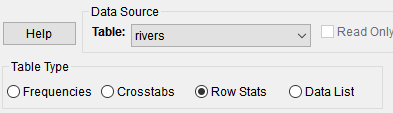
\includegraphics[]{gfx/cen005}}
      \caption{Central Measures for Rivers: Steps 1-2}
    \end{center}
  \end{figure}
  
  \item Columns: Add -> Length (Length)
  
  \begin{figure}[H]
    \begin{center}
      \fbox{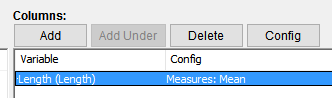
\includegraphics[]{gfx/cen010}}
      \caption{Central Measures for Rivers: Step 3}
    \end{center}
  \end{figure}
  
  \item Just above the ``Columns'' window, click the ``Config'' button and select: Mean, Median, and N.
  
  \begin{figure}[H]
    \begin{center}
      \fbox{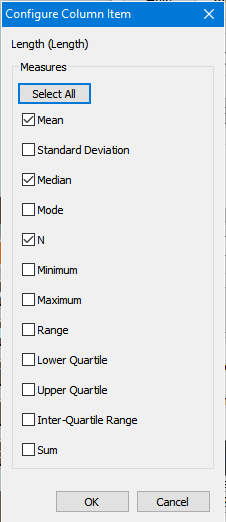
\includegraphics[]{gfx/cen015}}
      \caption{Central Measures for Rivers: Step 4}
    \end{center}
  \end{figure}
  
  \item Read those values in the lower left corner of the ``Make Report Table'' window.

  \begin{figure}[H]
    \begin{center}
      \fbox{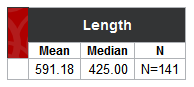
\includegraphics[]{gfx/cen020}}
      \caption{Central Measures for Rivers: Step 5}
    \end{center}
  \end{figure}

  \item Thus, there are $ 141 $ river lengths in the dataset, the mean length of those rivers is $ 591.18 $ miles and the median length is $ 425.00 $ miles. 
  
  \item To create a version of the output that can be saved and pasted into Word or some other program refer to the instructions in \nameref{app:b} (page \pageref{app:b}).

\end{enumerate}

\subsection{Activity 1: Central Measures} \label{cen:act01}

Using the \textit{maincafe} dataset in \texttt{SOFA} produce a table that contains the mean and median for Age, Bill, Length, and Miles data elements. The table should have a title of ``Central Measure, Activity 1'' and a subtitle of ``Main Street Cafe Central Measures''. 

\subsection{Grouping}

It is frequently desirable to group data so means can be compared. For example, it may be useful to group the mean of some variable by gender or some other category. To create groups in \texttt{SOFA}:

Start \texttt{SOFA} and select ``Report Tables.'' Then:

\begin{enumerate}
  \item Data Source Table: births
  \item Table Type: Row Stats
  \item Select ``Habit'' for the row
  \item Select ``Weeks,'' and ``Weight'' for Columns
  \item Click ``Config'' for each variable in Columns and select ``mean'' and ``median'' for those variables.
\end{enumerate}

\begin{figure}[H]
  \begin{center}
    \fbox{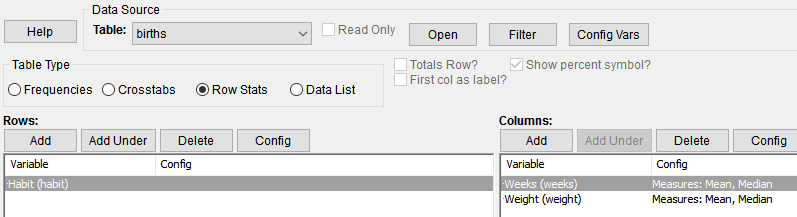
\includegraphics[width=\linewidth]{gfx/cen025}}
    \caption{Setting Up Groups of Central Measures}
  \end{center}
\end{figure}

Now, read the mean and median for weeks and weight grouped by smoking habit. 

\begin{figure}[H]
  \begin{center}
    \fbox{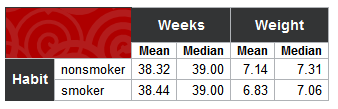
\includegraphics[]{gfx/cen030}}
    \caption{Central Measures for Weeks and Weight by Smoking Habit}
    \label{cen:img06}
  \end{center}
\end{figure}

In Figure \ref{cen:img06} the mean length of pregnancy, in weeks, for non-smokers is $ 38.32 $ and for smokers is $ 38.44 $. The mean and median for weight can also be easily read from the chart.

Sub-groups can also be created with \texttt{SOFA}. As an example, start \texttt{SOFA} and select ``Report Tables.'' Then:

\begin{enumerate}
  \item Data Source: births
  \item Table Type: Row Stats
  \item Click Add and then select ``Habit'' for the row
  \item For Rows, click ``Add Under'' and then select ``Gender'' 
  \item Select ``Weight'' for Columns
  \item Click ``Config'' for the columns and select ``mean'' and ``median''
\end{enumerate}

\begin{figure}[H]
  \begin{center}
    \fbox{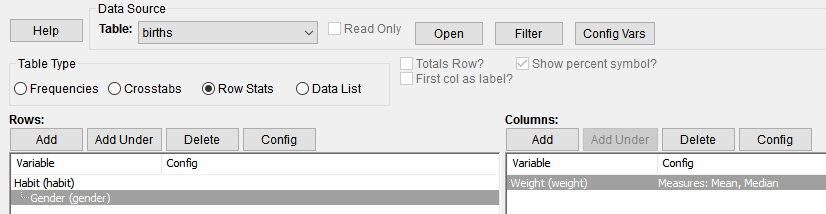
\includegraphics[width=\linewidth]{gfx/cen035}}
    \caption{Setting Up Subgroups}
  \end{center}
\end{figure}

\begin{figure}[H]
  \begin{center}
    \fbox{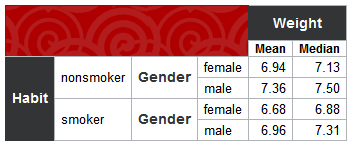
\includegraphics[]{gfx/cen040}}
    \caption{Mean and Median for Subgroups}
    \label{cen:img08}
  \end{center}
\end{figure}

In Figure \ref{cen:img08} female babies born to non-smokers have a mean weight of $ 6.94 $ pounds and females born to smokers have a mean weight of $ 6.68 $ pounds. 

To create meaningful statistics, the ``Row'' variables, which are used for grouping, should be either nominal or ordinal and the ``Column'' variables should be interval or ratio.

\subsection{Activity 2: Grouping} \label{cen:act02}

Using the \textit{maincafe} dataset in \texttt{SOFA} produce a table that contains the mean and median for Bill when grouped by Meal. The table should have a title of ``Central Measure, Activity 2'' and a subtitle of ``Main Street Cafe Grouped Central Measures''.

\subsection{Mode}

The mode is useful for dataset items that are nominal or ordinal in nature rather than interval or ratio. To find the mode for numeric data with \texttt{SOFA}:

Start \texttt{SOFA} and select ``Report Tables.'' Then:

\begin{enumerate}
  \item Data Source: births
  \item Table Type: Row Stats
  \item Columns: Add -> Visits
  \item Just above the ``Columns'' window, click the ``Config'' button and select: Mode.
  \item Read those values in the lower left corner of the ``Make Report Table'' window.
\end{enumerate}

\begin{figure}[H]
  \begin{center}
    \fbox{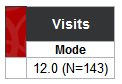
\includegraphics[]{gfx/cen045}}
    \caption{Mode for Visits}
  \end{center}
\end{figure}

$ 143 $ mothers visited the hospital $ 12 $ times, which is the mode for this data item and would be the best ``average'' to describe the number of hospital visits made by mothers.

If the data being analyzed is text rather than numeric then the mode must be found in a slightly different way. For example, the gender of the baby is listed in the dataset as ``male'' and ``female'' and \texttt{SOFA} will not calculate this mode since these are not numeric values. To find the mode for this type of data:

Start \texttt{SOFA} and select ``Report Tables.'' Then:

\begin{enumerate}
  \item Data Source: births
  \item Table Type: Row Stats
  \item Rows: Add -> Gender
  \item Columns: Add -> Sofa\_Id (Note: this is just a one-up number added by \texttt{SOFA} to each row of data as it is imported.)
  \item Just above the ``Columns'' window, click the ``Config'' button and select: N.
  \item The output table shows the frequency that each value appears in the dataset and the mode would be the largest of those frequencies.
\end{enumerate}

\begin{figure}[H]
  \begin{center}
    \fbox{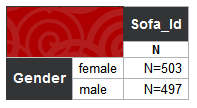
\includegraphics[]{gfx/cen050}}
    \caption{Mode for Baby Gender}
    \label{cen:img10}
  \end{center}
\end{figure}

For example, the information in Figure \ref{cen:img10} shows that there were more females than males in the dataset so that is the mode for Gender.

\subsection{Activity 3: Mode for Numeric Data} \label{cen:act03}

Using the \textit{maincafe} dataset in \texttt{SOFA} produce a table that contains the mode for both Food and Svc (these are ordinal data). The table should have a title of ``Central Measure, Activity 3'' and a subtitle of ``Main Street Cafe Food and Service Modes''.

\subsection{Activity 4: Mode for Text Data} \label{cen:act04}

Using the \textit{maincafe} dataset in \texttt{SOFA} produce a table that contains the mode for Day. The table should have a title of ``Central Measure, Activity 4'' and a subtitle of ``Main Street Cafe Day Mode''.

\section{Examples}

The following examples were created from the \textit{births} data and are provided for practice.

\begin{figure}[H]
  \begin{center}
    \fbox{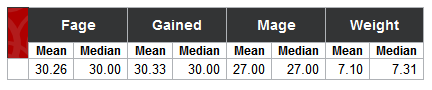
\includegraphics[]{gfx/cen055}}
    \caption{Various Means and Medians from the Births Data}
  \end{center}
\end{figure}

\begin{figure}[H]
  \begin{center}
    \fbox{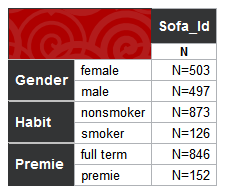
\includegraphics[]{gfx/cen060}}
    \caption{Various Modes from the Births Data}
  \end{center}
\end{figure}

\begin{figure}[H]
  \begin{center}
    \fbox{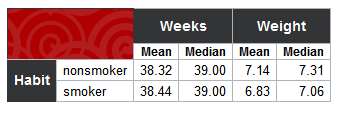
\includegraphics[]{gfx/cen065}}
    \caption{Length of Term and Baby's Weight Grouped by Smoker}
  \end{center}
\end{figure}

\section{Deliverable}

Complete the following activities in this lab:

\rowcolors{1}{gray!25}{}
\begin{center}
  \begin{tabular}{lll}
    \hline 
    \textbf{Number} & \textbf{Name} & \textbf{Page} \\ 
    \hline 
    \ref{cen:act01} & \nameref{cen:act01} & \pageref{cen:act01} \\ 
    \ref{cen:act02} & \nameref{cen:act02} & \pageref{cen:act02} \\ 
    \ref{cen:act03} & \nameref{cen:act03} & \pageref{cen:act03} \\ 
    \ref{cen:act04} & \nameref{cen:act04} & \pageref{cen:act04} \\ 
    \hline 
  \end{tabular} 
\end{center}

Screen capture the tables generated by each of these activities, add all of them into a single document, and submit that document for grading.